\section{Le système décimal}

% remarque : pour qu'un mot se retrouve dans le lexique : \MotDefinition{asymptote horizontale}{}
Les règles et conventions qui permettent d'écrire et de lire les nombres forment ce qu'on appelle un \textbf{système de numération}. Nous utilisons le système décimal, de base dix.

\begin{aconnaitre}
Pour écrire les chiffres dans le système décimal, il nous faut dix symboles, appelés des \emph{chiffres}. Ces chiffres sont :
\[ 0\,;\,1\,;\,2\,;\,3\,;\,4\,;\,5\,;\,6\,;\,7\,;\,8\,;\,9  \]
Il arrive parfois qu'on confonde \textbf{\MotDefinition{chiffre}{}} et \textbf{\MotDefinition{nombre}{}}. On peut faire l'analogie avec l'écriture d'une langue en affirmant que les \textbf{\textcolor{H1}{chiffres}} sont des \textbf{\textcolor{H1}{lettres}} et que les \textbf{\textcolor{H1}{nombres}} sont des \textbf{\textcolor{H1}{mots}}. Ainsi, 13 est un nombre qui s'écrit avec les chiffres 1 et 3.
\end{aconnaitre}

%%%%%%%%%%%%%%%%%%%%%%%%%%%%%%%%%%%%%%%%%%%%%%%%%%%%%%%%%%%%%%%%%%%%%%%%%%%
\prof
{Il est très important que les élèves fassent la différence entre chiffre et nombre pour la suite du chapitre. Ils ont sans doute appris autre chose à l'école primaire donc il faut dé-construire ce faux-savoir.}
%%%%%%%%%%%%%%%%%%%%%%%%%%%%%%%%%%%%%%%%%%%%%%%%%%%%%%%%%%%%%%%%%%%%%%%%%%%

Un \textbf{\textcolor{C2}{nombre décimal}} est un nombre qui s'écrit en deux parties séparées par une virgule (écriture décimale).

\hspace{2em}\textbullet\hspace{.25em} la partie entière, à gauche de la virgule. Elle correspond au nombre d'unités entières contenues dans le nombre.

\hspace{2em}\textbullet\hspace{.25em} la partie décimale, à droite de la virgule. Elle correspond à une portion d'unité supplémentaire.

De ce fait:

\begin{center}
\textbf{\textcolor{C2}{nombre décimal = partie entière + partie décimale}}
\end{center}

Un nombre entier est caractérisé par le fait qu'il n'a pas de partie décimale (on omet alors la virgule).


\begin{methode*1}[Tableau des nombres]
\begin{exemple*1}

Soit le nombre 34 567,19

\hspace{2em}\textbullet\hspace{.25em} Partie entière: 34 567
 
\hspace{2em}\textbullet\hspace{.25em} Partie décimale: 0,19


\end{exemple*1}

\exercice

Soit le nombre 10,153.

\hspace{2em}\textbullet\hspace{.25em}Partie entière: \dotfill

\hspace{2em}\textbullet\hspace{.25em} Partie décimale:\dotfill

\exercice

Compléter le tableau suivant pour les nombres 10,01 ; 0,037 ; 200 000 042 000.

\vspace{2em}

\begin{ttableau}{\linewidth}{19}
\hline
\multicolumn{3}{|c|}{milliards} & \multicolumn{3}{c|}{millions} & \multicolumn{3}{c|}{mille} & 
\multicolumn{3}{c|}{unités} & 
\multirow{2}{*}{\parbox{\linewidth}{ \vspace{1.5cm} \textcolor{B1}{  \textbf{,} }  }} &  %ADD PARBOX !!
\multirow{2}{*}{\rotatebox{90}{\phantom{dixièmes}}} &
\multirow{2}{*}{\rotatebox{90}{\phantom{centièmes}}} & 
\multirow{2}{*}{\rotatebox{90}{\phantom{millièmes}}} & 
\multirow{2}{*}{\rotatebox{90}{\phantom{dix-millièmes}}} & 
\multirow{2}{*}{\rotatebox{90}{\phantom{cent-millièmes}}} &
\multirow{2}{*}{\rotatebox{90}{\phantom{millionièmes}}} \\ \cline{1-12}
\rotatebox{90}{\phantom {centaines de ...}} & 
\rotatebox{90}{\phantom {dizaines de ...}} & 
\rotatebox{90}{\phantom {unités de ...}} &
\rotatebox{90}{\phantom {centaines de ...}} & 
\rotatebox{90}{\phantom {dizaines de ...}} & 
\rotatebox{90}{\phantom {unités de ...}} &
\rotatebox{90}{\phantom {centaines de ...}} & 
\rotatebox{90}{\phantom {dizaines de ...}} & 
\rotatebox{90}{\phantom {centaines de ...}} &
\rotatebox{90}{\phantom {dizaines de ...}} & 
\rotatebox{90}{\phantom {unités de ...}} & 
 & & & & & &       &   \\ \hline  % ADD EXTRA & ON THIS LINE B4 \\ \hline !!
& & & & & 3 & 0 & 2 & 7 & 4 & 6 & 2 & \textcolor{B1}{\textbf{,}} & 0 & 0 & 0 & 0 & 0 & 0 \\ \hline
& & & & & & & & & & & & \textcolor{B1}{\textbf{,}} & & & & & &\\ \hline
& & & & & & & & & & & & \textcolor{B1}{\textbf{,}} & & & & & &\\ \hline
& & & & & & & & & & & & \textcolor{B1}{\textbf{,}} & & & & & &\\ \hline
\end{ttableau}
\end{methode*1}

\begin{remarque}

\hspace{2em}\textbullet\hspace{.25em} La partie décimale est toujours finie: on peut compter les chiffres après la virgule.

\hspace{2em}\textbullet\hspace{.25em} Lorsque la partie décimale n'est pas finie, on a un nombre infini qui n'est PAS un nombre décimal.

\hspace{2em}\textbullet\hspace{.25em} Lorsque la partie décimale ne comporte que des 0, on les supprime avc la virgule et on parle alors de \textbf{\textcolor{C2}{nombre entier}}.
\end{remarque}
%%%%%%%%%%%%%%%%%%%%%%%%%%%%%%%%%%%%%%%%%%%%%%%%%%%%%%%%%%%%%%%%%%%%%%%%%%%

\section{Nombre en écriture fractionnaire}
Le système décimal peut se représenter ainsi:

\begin{center}
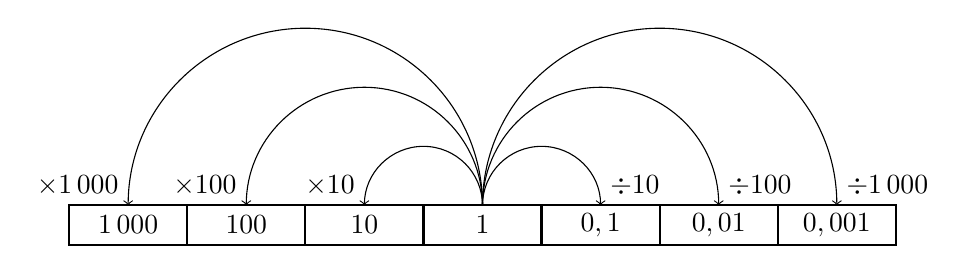
\begin{tikzpicture}[scale=0.5]
\foreach \x in {0,1,...,6} \draw[thick] (-1.5+3*\x,-0.5) rectangle (1.5+3*\x,0.5);
\draw (0,0) node {$1\,000$};
\draw (3,0) node {$100$};
\draw (6,0) node {$10$};
\draw (9,0) node {$1$};
\draw (12,0) node {$0,1$};
\draw (15,0) node {$0,01$};
\draw (18,0) node {$0,001$};
\draw[->] (9,0.5) arc (0:180:4.5) node[above left] {$\times 1\,000$};
\draw[->] (9,0.5) arc (0:180:3) node[above left] {$\times 100$};
\draw[->] (9,0.5) arc (0:180:1.5) node[above left] {$\times 10$};

\draw[->] (9,0.5) arc (180:0:4.5) node[above right] {$\div 1\,000$};
\draw[->] (9,0.5) arc (180:0:3) node[above right] {$\div 100$};
\draw[->] (9,0.5) arc (180:0:1.5) node[above right] {$\div 10$};
\end{tikzpicture}
\end{center}

Dans la partie entière $\left\lbrace
	\begin{matrix}
	\text{Une dizaine c'est l'unité prise 10 fois.}\\
	\text{Une centaine c'est l'unité prise 100 fois.}\\
	\text{Un millier c'est l'unité prise 1 000 fois.}\\
	\end{matrix}
\right.$ 

Dans la partie décimale $\left\lbrace
	\begin{matrix}
	\text{Une dixième c'est l'unité divisée par 10. Cela peut s'écrire} \frac{1}{10}. \\
	\text{Un centième c'est l'unité divisée par 100. Cela peut s'écrire} \frac{1}{100}. \\
	\text{Un millième c'est l'unité divisée par 1 000. Cela peut s'écrire} \frac{1}{1000}.
	\end{matrix}
\right.$

		\subsection{Ecriture fractionnaire d'un nombre}
\begin{aconnaitre}
Le "partage" de l'unité peut s'écrire \textbf{sous forme fractionnaire}.

Ainsi $\frac{1}{5}$ se lit "un cinquième". Cette fraction représente l'unité divisée en 5 parts égales. \\

\begin{center}
\begin{tikzpicture}[scale=0.5]
\fill[white] (0,0) rectangle (5,5);        % Specify colour
\fill[gray!40] (0,0) rectangle (1,5);        % Specify colour
\draw[thick] (0,0) -- (5,0) -- (5,5) -- (0,5) -- cycle;
\foreach \x in {1,2,3,4} \draw[thick] (\x,0) -- (\x,5);

\draw (2.5,0) node[below] {$\dfrac{1}{5}=0,2$};
\end{tikzpicture}
\end{center}

$\frac{1}{5}$ est \textbf{l'écriture fractionnaire} alors que 0,2 est \textbf{l'écriture décimale} \underline{d'une même quantité}.
\end{aconnaitre}

\begin{methode*1}[Comprendre les fractions]
	\begin{exemple*1}
\vspace{0.5cm}	
	
Dans le nombre $\frac{3}{5}$ l'unité est divisée en 5 parts égales et on a pris trois parts: $3\times \frac{1}{5}$.
\begin{center}
\begin{tikzpicture}[scale=0.5]
\fill[white] (0,0) rectangle (5,5);        % Specify colour
\fill[gray!40] (0,0) rectangle (3,5);        % Specify colour
\draw[thick] (0,0) -- (5,0) -- (5,5) -- (0,5) -- cycle;
\foreach \x in {1,2,3,4} \draw[thick] (\x,0) -- (\x,5);

\draw (2.5,0) node[below] {$\dfrac{3}{5}=0,6$};
\end{tikzpicture}
\end{center}

Le nombre du bas, celui qui indique le nombre de parts dans l'unité, s'appelle \textbf{\textcolor{C2}{le dénominateur}}.\\
Le nombre du haut, celui qui indique le nombre de parts, s'appelle \textbf{\textcolor{C2}{le numérateur}}.
\end{exemple*1}

\exercice

Dans chaque cas, donner l'écriture décimale correspondante:

$\frac{1}{100}$=\dotfill \\
$\frac{3}{4}$=\dotfill \\
$\frac{7}{10}$=\dotfill \\
$\frac{12}{25}$=\dotfill \\
$\frac{23}{50}$=\dotfill

\exercice

Dans chaque cas, donner une écriture fractionnaire correspondante:

0,5=\dotfill \\
0,32=\dotfill \\
0,04=\dotfill \\
0,25=\dotfill

\end{methode*1}

\begin{remarque}
Il est important de savoir calculer avec des écritures fractionnaires car certaines quantités ne peuvent pas s'écrire sous forme décimale.\end{remarque}

		\subsection{Partie entière et nombres en écriture fractionnaire}

Parfois, il arrive qu'on "garde" tellement de morceaux d'unité, qu'on arrive à reconstituer une ou plusieurs unités.

\begin{methode*1}[Fraction supérieure à 1]
	\begin{exemple*1}
\vspace{0.5cm}	
	
Prenons la fraction: $\frac{12}{5}$.\\
Cela signifie qu'on a gardé 12 parts égales à $\frac{1}{5}$.\\
Avec 5 parts égales à $\frac{1}{5}$, on peut faire une unité. Donc avec 12 parts de $\frac{1}{5}$, on peut constituer 2 unités et il restera 2 parts de $\frac{1}{5}$ c'est à dire $\frac{2}{5}$.\\
On peut donc dire que $\frac{12}{5}$=2+$\frac{2}{5}$=2,4.

\begin{center}
\begin{tikzpicture}[scale=0.5]
\fill[white] (0,0) rectangle (5,5);        % Specify colour
\fill[gray!40] (0,0) rectangle (5,5);        % Specify colour
\draw[thick] (0,0) -- (5,0) -- (5,5) -- (0,5) -- cycle;
\foreach \x in {1,2,3,4} \draw[thick] (\x,0) -- (\x,5);

\fill[white] (6,0) rectangle (11,5);        % Specify colour
\fill[gray!40] (6,0) rectangle (11,5);        % Specify colour
\draw[thick] (6,0) -- (11,0) -- (11,5) -- (6,5) -- cycle;
\foreach \x in {1,2,3,4} \draw[thick] (6+\x,0) -- (6+\x,5);

\fill[white] (12,0) rectangle (17,5);        % Specify colour
\fill[gray!40] (12,0) rectangle (14,5);        % Specify colour
\draw[thick] (12,0) -- (17,0) -- (17,5) -- (12,5) -- cycle;
\foreach \x in {1,2,3,4} \draw[thick] (12+\x,0) -- (12+\x,5);

\draw (8.5,0) node[below] {$\dfrac{12}{5}=2,4$};
\end{tikzpicture}
\end{center}

\end{exemple*1}

\exercice

Dans chaque cas, écrire la fraction sous forme d'une somme d'un entier et d'une autre fraction inférieure à 1 puis sous la forme d'un nombre décimal.

$\frac{6}{4}$=1+$\frac{2}{4}$=1,5\\
$\frac{9}{2}$=\dotfill \\
$\frac{35}{10}$=\dotfill \\
$\frac{17}{5}$=\dotfill \\
$\frac{143}{100}$=\dotfill

\end{methode*1}

%%%%%%%%%%%%%%%%%%%%%%%%%%%%%%%%%%%%%%%%%%%%%%%%%%%%%%%%%%%%%%%%%%%%%%%%%%%

\section{Droite ou axe gradué}

\begin{aconnaitre}
Les \textbf{\textcolor{C2}{nombres entiers}}
peuvent être placés sur une droite ou un axe. A chaque point de la droite, on associe un nombre: c'est l'abscisse du point.
\end{aconnaitre}
\begin{methode*1}[Repérer sur une demi-droite graduée]
	\begin{exemple*1}

\vspace{0.5cm}

 
 L'abscisse du point $F$ est $\frac{1}{5}=0,2$ donc on note F(0,2).
 
 L'abscissedu point $G$ est $\frac{6}{5}=6 \times0,2=1,2$ donc on note G(1,2).
 
 L'abscisse du point $H$ est $\frac{11}{5}=11 \times0,2=2,2$ donc on note H(2,2).
   
 
\tikzset{
   cross/.pic = {
     \draw[thick] (-0.2,0.2) -- (0.2,-0.2);
     \draw[thick] (-0.2,-0.2) -- (0.2,0.2);}
}

\begin{tikzpicture}[general]
% The axis
\draw[decoration={markings,mark=at position 1 with
    {\arrow[scale=3]{>}}},postaction={decorate}] (0,0) -- (12,0); 
% The ticks
\foreach \x in {0,...,11} \draw (\x,-0.2) -- (\x,0.2);
\foreach \x in {0,1,2} \draw (5*\x,-0.35) -- (5*\x,0.35);
% The numbers
\draw (0,-0.35) node[below] {\large $0$};
\draw (5,-0.35) node[below] {\large $1$};
% The markers
\pic[scale=0.6] at (1,0) {cross}; \draw (1,0.5) node {\large $F$};
\pic[scale=0.6] at (6,0) {cross}; \draw (6,0.5) node {\large $G$};
\pic[scale=0.6] at (11,0) {cross}; \draw (11,0.5) node {\large $H$};
\end{tikzpicture}
\end{exemple*1}

\begin{remarque}
Il arrive parfois que les graduations de l'axe ne commencent pas à 0 ou que l'axe ne soit pas gradué de 1 en 1. Dans ce cas, il s'agit de repérer la valeur d'\textbf{une} graduation grâce aux valeurs données.
\end{remarque}

\exercice

\tikzset{
   cross/.pic = {
     \draw[thick] (-0.2,0.2) -- (0.2,-0.2);
     \draw[thick] (-0.2,-0.2) -- (0.2,0.2);}
}

\begin{tikzpicture}[general]
% The axis
\draw[decoration={markings,mark=at position 1 with
    {\arrow[scale=3]{>}}},postaction={decorate}] (-0.8,0) -- (11.5,0); 
% The ticks
\foreach \x in {1,...,11} \draw (0.8*\x,-0.2) -- (0.8*\x,0.2);
\foreach \x in {0,1,...,6} \draw (0.8*2*\x,-0.35) -- (0.8*2*\x,0.35);
% The numbers
%\draw (0,-0.35) node[below] {\large $0$};
%\draw (5,-0.35) node[below] {\large $50$};
% The markers
\pic[scale=0.6] at (0,0) {cross}; \draw (0,0.5) node {\large $P$};
\pic[scale=0.6] at (0.8*5,0) {cross}; \draw (0.8*5,0.5) node {\large $S$};
%\pic[scale=0.6] at (0.8*8,0) {cross}; 
\draw (0.8*8,-0.6) node {\large $800$};
\draw (0.8*12,-0.6) node {\large $1\,000$};
\pic[scale=0.6] at (0.8*13,0) {cross};  \draw (0.8*13,0.5) node {\large $R$};
\end{tikzpicture}

Ici, de 800 à 1000, il y a \dotfill graduations. Donc chaque graduation représente \dotfill .

L'abscisse du point \dotfill est \dotfill donc on note \dotfill. 

L'abscisse du point \dotfill est \dotfill donc on note \dotfill. 

L'abscisse du point \dotfill est \dotfill donc on note \dotfill. 
\end{methode*1}

%%%%%%%%%%%%%%%%%%%%%%%%%%%%%%%%%%%%%%%%%%%%%%%%%%%%%%%%%%%%%%%%%%%%%%%%%%%
\section{Travail sur les nombres: encadrer et arrondir}

% remarque : pour qu'un mot se retrouve dans le lexique : \MotDefinition{asymptote horizontale}{} 


\begin{aconnaitre}
\textbf{\MotDefinition{Encadrer}{}} un nombre, c'est trouver un nombre qui est plus petit que lui et un nombre qui est plus grand que lui. On écrit un encadrement avec les symboles $<$ ; $\leqslant$ ; $>$ et $\geqslant$. 
\end{aconnaitre}


\begin{methode*1}[Encadrer]

\begin{exemple*1}
Encadrer 13,345 à l'unité puis au centième.\\[0.5em]
Pour encadrer à l'unité, on «coupe» le nombre 13,345 à l'unité: 13.\
13 est plus petit  que 13,345 qui est plus petit que 14 (on ajoute une \textbf{unité}) .\
On écrit alors : $13 < 13,345 < 14$. \\[1em]
Pour encadrer au centième, on «coupe» le nombre 13,345 au centième: 13,34.\
13,34 est plus petit que 13,345 qui est plus grand que 13,35 (on ajoute un \textbf{centième}).\
On écrit alors : $13,34 < 13,345 < 13,35$.
\end{exemple*1}

\exercice

Encadrer les nombres 237,48 et 43,923\,5 à la dizaine puis au centième.
%\correction

\end{methode*1}

%%%%%%%%%%%%%%%%%%%%%%%%%%%%%%%%%%%%%%%%%%%%%%%%%%%%%%%%%%%%%%%%%%%%%%%%%%


\begin{aconnaitre}
\textbf{\MotDefinition{Arrondir}{}} un nombre, c’est le remplacer par le nombre le plus proche à la précision désirée. Pour cela:
\begin{itemize}
 \item on encadre le nombre à la précision demandée ;
 \item on choisit la valeur (inférieure ou supérieure) qui est la plus proche du nombre d'origine.
 \end{itemize}
 
On peut aussi regarder comment le nombre est formée:
\begin{itemize}
\item on choisit le dernier chiffre à conserver;
 \item on conserve ce chiffre si le suivant est 0, 1, 2, 3 ou 4 ;
 \item on augmente de 1 ce chiffre si le suivant est 5, 6, 7, 8, ou 9.
 \end{itemize}
\end{aconnaitre}


\begin{methode*1}[Arrondir]

\begin{exemple*1}
Donner l'arrondi \textbf{à l'unité} de 73,2.\\
\begin{tikzpicture}
%Background in white
\fill[fill=white] (-1.0,-2.5) rectangle (11.5,2.5);
\foreach \n in {6, 5, ..., 0}
	\draw (0.2*\n,0.1*\n) node {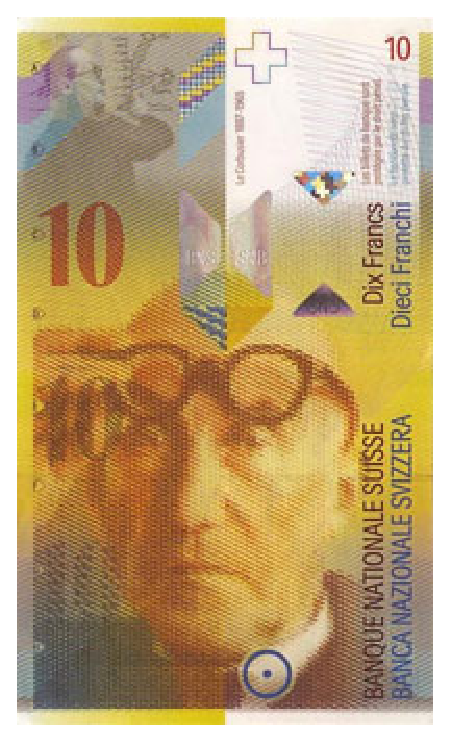
\includegraphics[width=1.5cm]{SF10}};
\foreach \n in {0,1,2}
	\draw (2.3,0.5*\n+0.5) node {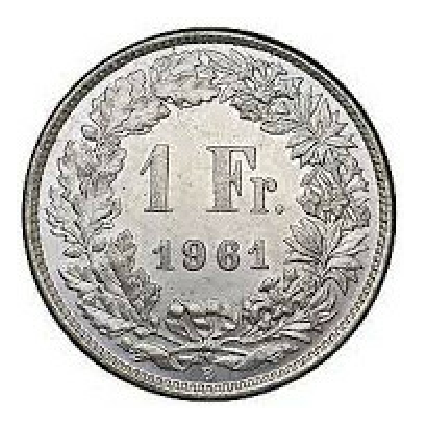
\includegraphics[width=0.5cm]{SF1}};

\draw (0, -1.75) node{\scalebox{1.5}{$73$}};

%Offset 1: 4cm
\foreach \n in {6, 5, ..., 0}
	\draw (4+0.2*\n,0.1*\n) node {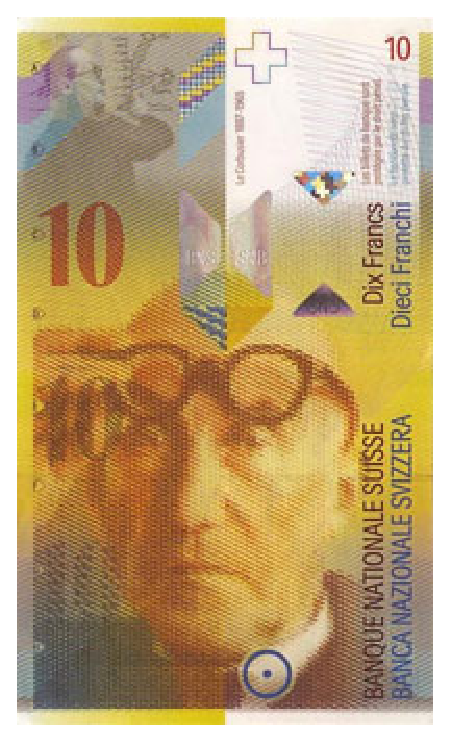
\includegraphics[width=1.5cm]{SF10}};
\foreach \n in {0,1,2}
	\draw (4+2.3,0.5*\n+0.5) node {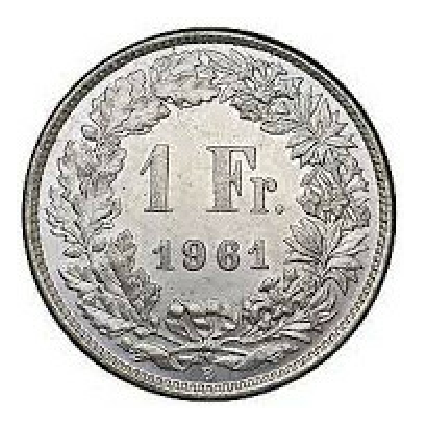
\includegraphics[width=0.5cm]{SF1}};
\foreach \n in {0,1}
	\draw (4+2.8,0.25*\n+1.4) node {
\includegraphics[width=0.25cm]{centimes10}};

\draw (4, -1.75) node{\scalebox{1.5}{$73,20$}};


%Offset 2: 8cm
\foreach \n in {6, 5, ..., 0}
	\draw (8.5+0.2*\n,0.1*\n) node {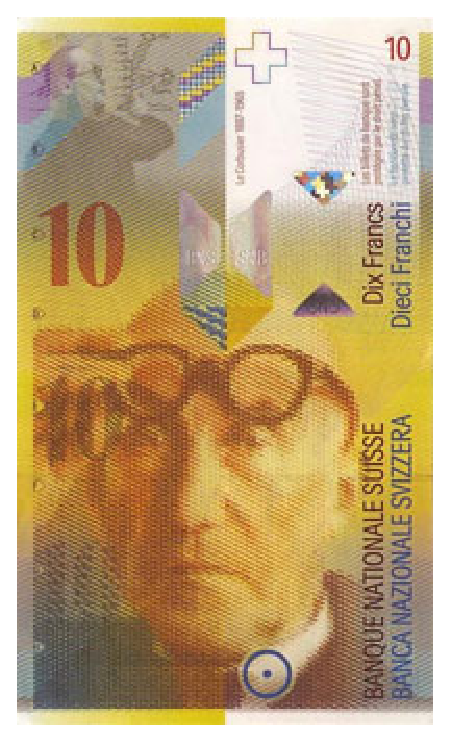
\includegraphics[width=1.5cm]{SF10}};
\foreach \n in {0,1,2,3}
	\draw (8.5+2.3,0.5*\n) node {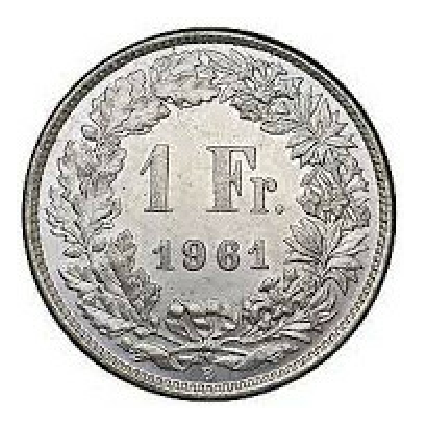
\includegraphics[width=0.5cm]{SF1}};

\draw (8.5, -1.75) node{\scalebox{1.5}{$74$}};


\draw (2.9,0.5) node {\scalebox{2}{$<$}};
\draw (7.4,0.5) node {\scalebox{2}{$<$}};

%\draw (1,0.1) node {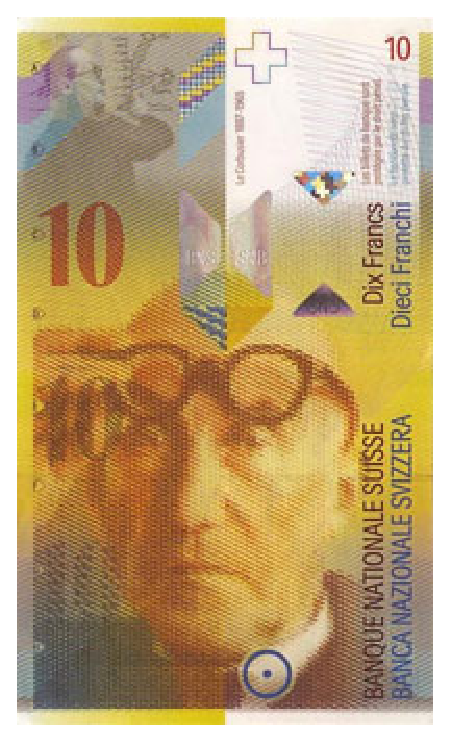
\includegraphics[width=3cm]{SF10}};
%\draw (2,3) node {
\includegraphics[width=0.75cm]{centimes10}};
\end{tikzpicture}


Donner l'arrondi \textbf{à l'unité} de 126,5.\\
%%%%%%%%%%%%%Illustration Paul


Donner l'arrondi \textbf{au centième} de 2,38.\\
%\def\euroneoff{2}
\begin{tikzpicture}
\fill[fill=white] (-1.0,-1.6) rectangle (11.5,1.8);

% 2,30
\foreach \n in {0,1}
	\draw (0+0.5,\n)  node {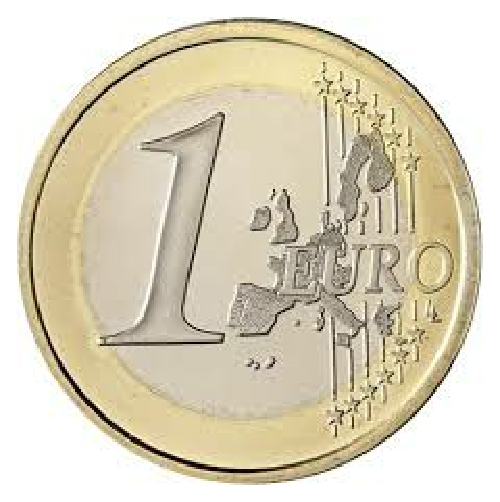
\includegraphics[width=1cm]{euro1}};

\foreach \n in {0,1,2}
	\draw (0.9+0.5,\n*0.6) node {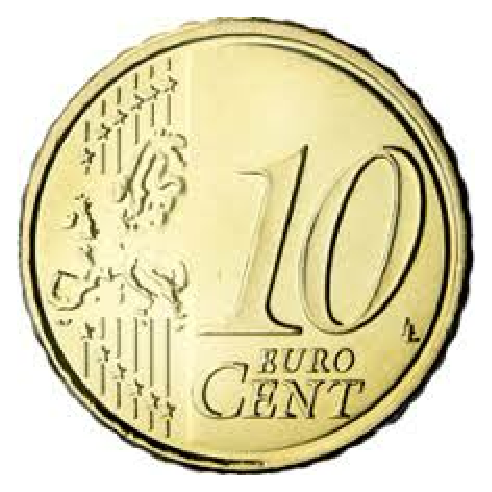
\includegraphics[width=0.6cm]{centimes10eur}};

\draw (0+0.5, -1.25) node{\scalebox{1.5}{$2,30$}};

% 2,38
\foreach \n in {0,1}
	\draw (3.5,\n)  node {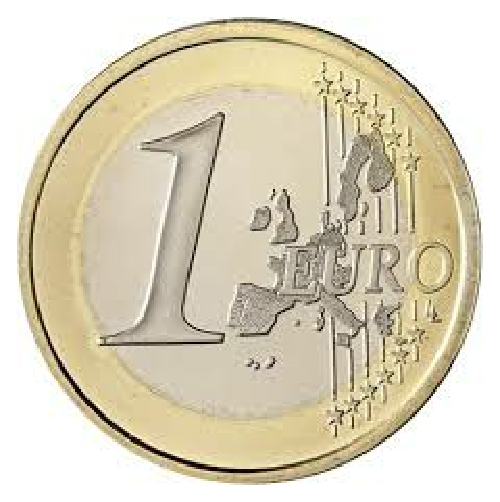
\includegraphics[width=1cm]{euro1}};
\foreach \n in {0,1,2}
	\draw (3.5+0.9,\n*0.6) node {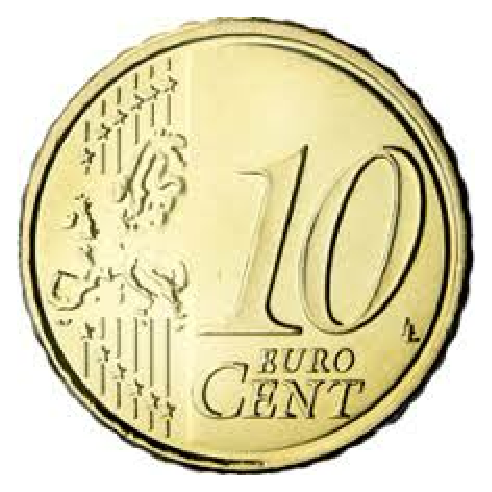
\includegraphics[width=0.6cm]{centimes10eur}};

\foreach \n in {0,1,2}
	\draw (3.5+1.5,0.475+\n*0.4) node {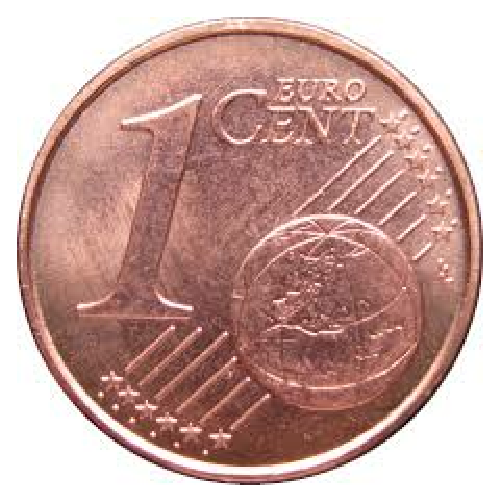
\includegraphics[width=0.4cm]{centime1eur}};
\foreach \n in {0,1,2}
	\draw (3.5+1.5+0.5,0.475+\n*0.4) node {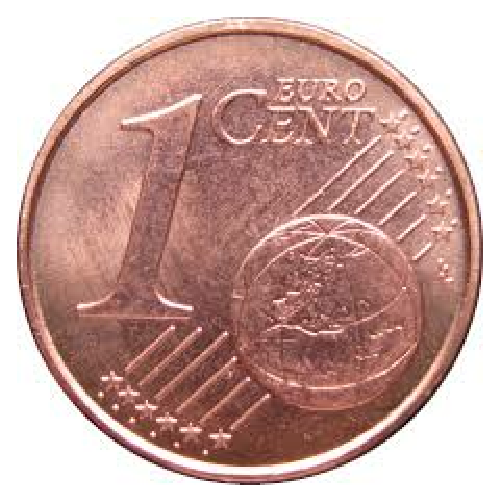
\includegraphics[width=0.4cm]{centime1eur}};
\foreach \n in {0,1}
	\draw (3.5+1.5+1 ,0.475+\n*0.4+0.4) node {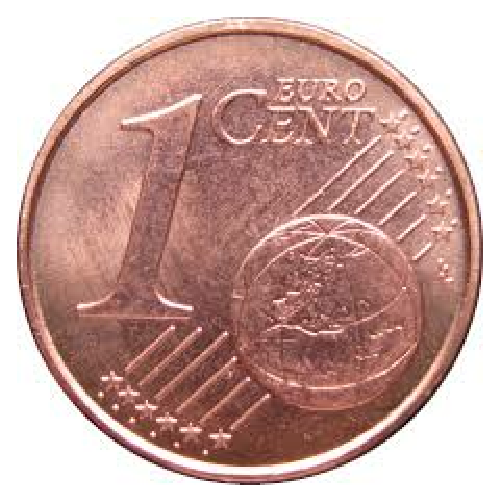
\includegraphics[width=0.4cm]{centime1eur}};

\draw (3.5, -1.25) node{\scalebox{1.5}{$2,38$}};


% 2.40
\foreach \n in {0,1}
	\draw (8,\n)  node {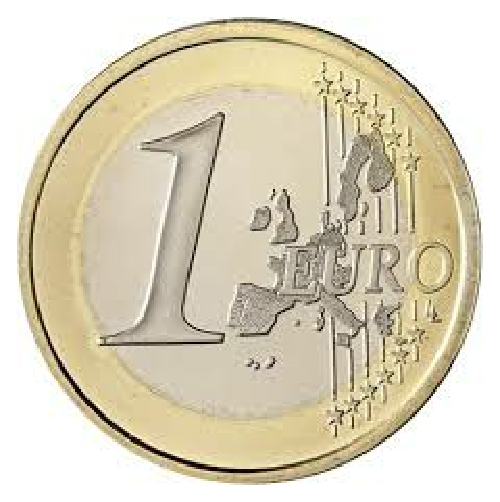
\includegraphics[width=1cm]{euro1}};
\foreach \n in {0,1,2,3}
	\draw (8+0.9,\n*0.6-0.6) node {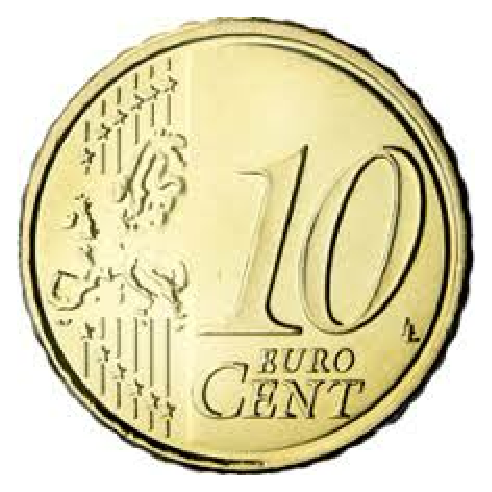
\includegraphics[width=0.6cm]{centimes10eur}};

\draw (8, -1.25) node{\scalebox{1.5}{$2,40$}};

\draw (2.4,0.5) node {\scalebox{2}{$<$}};
\draw (6.9,0.5) node {\scalebox{2}{$<$}};

\end{tikzpicture}


Donner l'arrondi \textbf{au centième} de 12,543.\\
%%%%%%%%%%%%%Illustration Paul

\end{exemple*1}

\exercice

Arrondir à l'unité les nombres 1247,20 et 25,385. Arrondir au dixième les nombres 1,99 et 3,14159.

%\correction

\end{methode*1}
